\let\negmedspace\undefined
\let\negthickspace\undefined
\documentclass[journal]{IEEEtran}
\usepackage[a5paper, margin=10mm, onecolumn]{geometry}
%\usepackage{lmodern} % Ensure lmodern is loaded for pdflatex
\usepackage{tfrupee} % Include tfrupee package

\setlength{\headheight}{1cm} % Set the height of the header box
\setlength{\headsep}{0mm}     % Set the distance between the header box and the top of the text

\usepackage{gvv-book}
\usepackage{gvv}
\usepackage{cite}
\usepackage{amsmath,amssymb,amsfonts,amsthm}
\usepackage{algorithmic}
\usepackage{graphicx}
\usepackage{textcomp}
\usepackage{xcolor}
\usepackage{txfonts}
\usepackage{listings}
\usepackage{enumitem}
\usepackage{mathtools}
\usepackage{gensymb}
\usepackage{comment}
\usepackage[breaklinks=true]{hyperref}
\usepackage{tkz-euclide} 
\usepackage{listings}
% \usepackage{gvv}                                        
\def\inputGnumericTable{}                                 
\usepackage[latin1]{inputenc}                                
\usepackage{color}                                            
\usepackage{array}                                            
\usepackage{longtable}                                       
\usepackage{calc}                                             
\usepackage{multirow} 
\usepackage{hhline}                                           
\usepackage{ifthen}                                           
\usepackage{lscape}
\usepackage{circuitikz}
\tikzstyle{block} = [rectangle, draw, fill=blue!20, 
    text width=4em, text centered, rounded corners, minimum height=3em]
\tikzstyle{sum} = [draw, fill=blue!10, circle, minimum size=1cm, node distance=1.5cm]
\tikzstyle{input} = [coordinate]
\tikzstyle{output} = [coordinate]

\begin{document}
\bibliographystyle{IEEEtran}
\vspace{3cm}

\title{MatGeo Assignment 3.2.23}
\author{AI25BTECH11007}
 \maketitle
% \newpage
% \bigskip
{\let\newpage\relax\maketitle}

\renewcommand{\thefigure}{\theenumi}
\renewcommand{\thetable}{\theenumi}
\setlength{\intextsep}{10pt} % Space between text and floats


\numberwithin{equation}{enumi}
\numberwithin{figure}{enumi}
\renewcommand{\thetable}{\theenumi}
\textbf{Question:}\\

Construct a triangle $ABC$ in which 
\[
BC = 5 \,\text{cm}, \quad \angle B = 60^\circ, \quad \text{and} \quad AC + AB = 7.5 \,\text{cm}.
\]


\textbf{Solution:}\\

Using the cosine formula in $\triangle ABC$,
\begin{align}
\textbf{Cosine Formula :   } 
    b^{2} &= a^{2} + c^{2} - 2ac\cos B \\
\Rightarrow (7.5-c)^{2} &= 5^{2} + c^{2} - 2\cdot 5c \cos 60^\circ \\
\Rightarrow c &= \frac{7.5^{2}-5^{2}}{2(7.5-5\cos 60^\circ)} 
\end{align}

\[
c = 3.125, 
\qquad b = 7.5 - 3.125 = 4.375.
\]

The coordinates of $\triangle ABC$ can then be expressed as
\[
A=\myvec{\tfrac{3.125\cos 60^\circ}{\sin 60^\circ}\\[6pt]\tfrac{3.125}{\sin 60^\circ}},\quad 
B=\myvec{0\\0},\quad 
C=\myvec{5\\0}.
\]

The coordinates of $\triangle ABC$ are
\[
A=\myvec{\tfrac{3.125}{\sqrt{3}} \\[6pt] \tfrac{6.25}{\sqrt{3}}}
\;\approx\;
\myvec{1.804 \\[6pt] 3.608},\quad
B=\myvec{0 \\ 0},\quad
C=\myvec{5 \\ 0}.
\]

\begin{figure}[H]
    \centering
    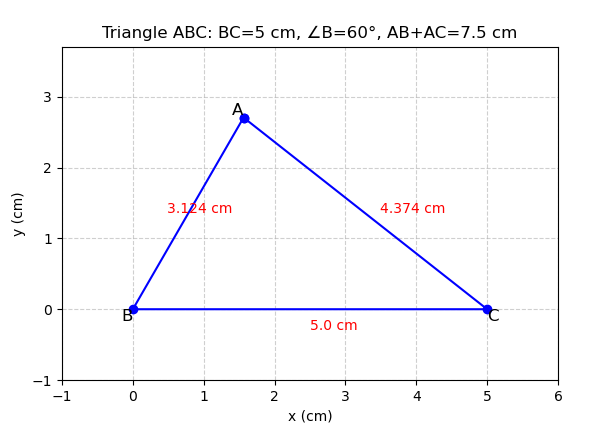
\includegraphics[width=1.0\linewidth]{figs/image.png}
    \caption{Construction Plot}
    \label{fig:placeholder}
\end{figure}

\end{document}